\documentclass{article}
\usepackage[a4paper left=1in, right=1in, top=1in, bottom=1in]{geometry}
\usepackage{tikz}
\usetikzlibrary{positioning}

\begin{document}
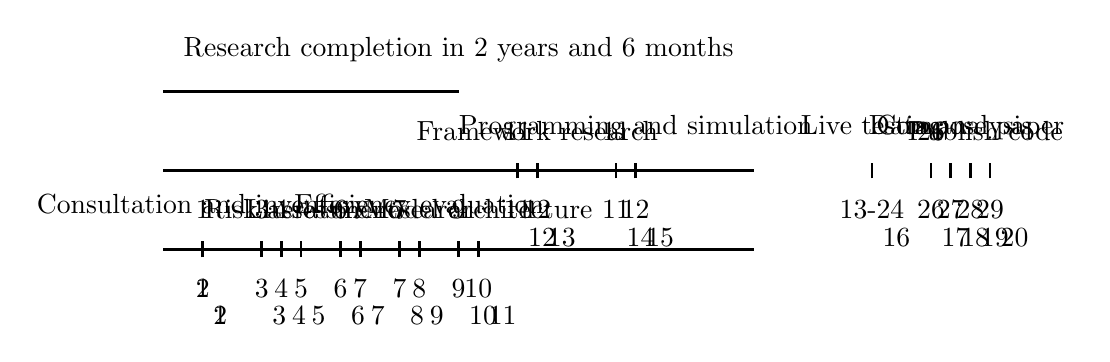
\begin{tikzpicture}[x=0.25cm, y=0.5cm, line width=1pt]

% Horizontal lines
\draw (0,0) -- (30,0);
\draw (0,2) -- (30,2);
\draw (0,4) -- (15,4);

% Timeline entries
\foreach \x/\month/\activity [count=\i] in {
    2/1,2/2/Consultation and inventory,
    5/3,6/4,7/5/Risk assessment,
    9/6,10/7/Literature research,
    12/7,13/8/Efficiency evaluation,
    15/9,16/10/Model architecture,
    18/11,19/12/Framework research,
    23/11,24/12/Programming and simulation,
    36/13-24/Live testing,
    39/26,40/27/Data analysis,
    41/28/Compose paper,
    42/29/Publish code
  }
{
  % Calculate x position with event spacing
  \pgfmathsetmacro\xpos{\x}

  % Determine y position based on the year
  \pgfmathsetmacro\ypos{floor(\i/12)*2}

  % Tick mark
  \draw (\xpos,\ypos-0.2) -- (\xpos,\ypos+0.2);

  % Month label
  \node[anchor=north] at (\xpos,\ypos-0.5) {\month};

  % Activity label
  \node[anchor=south, align=center] at (\xpos,\ypos+0.5) {\activity};
  
  % Activity number
  \node[anchor=north west] at (\xpos, \ypos-1.2) {\i};
}

% Timeline completion estimation
\node[anchor=south] at (15, 4.5) {Research completion in 2 years and 6 months};

\end{tikzpicture}
\end{document}